\section{Infrastruktur}
\label{sec:recorder}
\begin{figure}
    \centering
    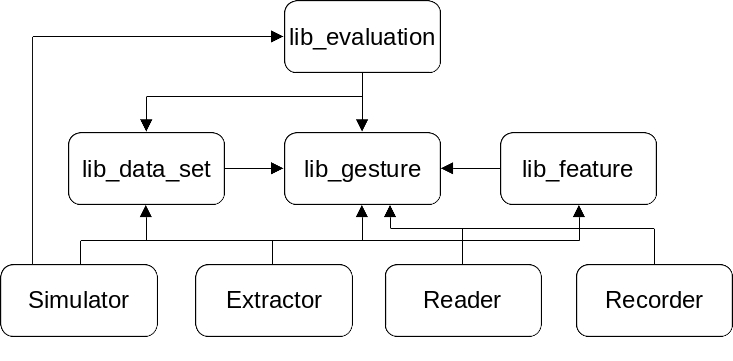
\includegraphics[width=0.75\linewidth]{images/architecture_overview.jpg}
    \caption{Abhängigkeitein der einzelnen Module.}
    \label{fig:architecture_overview}
\end{figure}
In dieser Arbeit mussten viele Features und Konfigurationen der Entscheidungsbäume untersucht und zu getestet werden. Aus diesem Grund wurde eine umfangreiche Infrastruktur geschaffen, die die
Auswertung von ML Modellen mit den Handgestendaten vereinfacht. Die Infrastruktur umfasst ein Datenmodel für Handgesten und kann die Datenmengen mit verschiedenen Parsingmethoden einlesen.
\newline
\newline
Außerdem können synthetischen Daten auf verschiedene Arten generiert werden. Die Architektur der Infrakstruktur erlaubt es weitere Features hinzuzufügen, ohne Kompatibilitätsprobleme zu verursachen.
Alle Funktionalitäten sind in Code-Bibliotheken isoliert, um die Integration in Hilfprogramme zu vereinfachen (siehe Abbildung \ref{fig:architecture_overview}).
\newline
\newline
Im folgenden wird die Funktionalität der einzelnen Module vorgestellt und die daraus erstellten Hilfsprogramme.
\newline
\newline
\texttt{lib\_gesture} definiert die Handgeste und die vorhandenen Gestentypen. Außerdem implementiert sie zwei Parsing-Methoden. Die erste Methode parsed Handgesten nach Annotation und die
zweite nach Kubiks Algorithmus (siehe Sektion \ref{sec:gesture_extraction}). Die Handgeste selber implementiert Methoden um synthetische Daten zu generieren.
\begin{itemize}
    \item Rotation um 90°, 180° und 270°.
    \item Nullgesten durch das Kombinieren der ersten Hälfte der Ausgangsgeste und der zweiten Hälfte von dessen Rotationen.
    \item Verschiebung der Pixel nach Oben und Unten für eine Links nach Rechts bzw. Rechts nach Links Geste und analog dazu eine Verschiebung nach Links und Rechts für die restlichen Handgesten.
    \item Rotation der äußeren Pixel um Diagonale Handgesten zu generieren.
\end{itemize}
\begin{lstlisting}[label=lst:FeatureInterface,caption={Interface, um ein Feature zu implementieren.}]
pub trait Feature {
    fn calculate(gesture: &Gesture) -> Self where Self: Sized;
    fn marshal(&self) -> String;
}
\end{lstlisting}
\texttt{lib\_feature} bietet ein einfaches Interface an um Feature mit einer Handgeste (siehe Listing \ref{lst:FeatureInterface}) zu implementieren. Zurzeit sind 28 verschiedene Feature implementiert.
\newline
\newline
\texttt{lib\_data\_set} stellt alle verfügbaren Datenmengen als statische Importe bereit. Einträge sind bereits nach Distanz zur Kamera, Helligkeit, Verdeckungsobjekt und Ausführungsgeschwindigkeit klassifiziert. Ein
Eintrag kann in der Helligkeit verändert werden entweder durch einen Offset oder indem er skaliert wird.
\newline
\newline
\texttt{lib\_evaluation} bietet ein Hilfsobjekt an, dass Datenmengen nach Erkennungsgenauigkeit auswertet und Berichte daraus generiert.
\newline
\newline
Der \texttt{Simulator} ist zweigeteilt. Der aktive Teil nutzt die die Gestenkandidatenerkennungsmethode nach Kubik, die in \texttt{lib\_gesture} implementiert ist, um den seriellen Datenstrom des Arduino zu parsen. Der
Gestenkandidat wird anschließend durch das hinterlegte Model klassifiziert und das Ergebnis ausgegeben. Der passive Teil evaluiert die Erkennungsgenauigkeit aller definierten Datenmengen.
\newline
\newline
Der \texttt{Extractor} extrahiert aus spezifizierten Datenmengen die definierten Features und exportiert diese in Dateien, sodass sie von dem Model zum Trainieren genutzt werden können. Optional kann die Datenmenge durch
sythetische Daten erweitert werden.
\newline
\newline
Der \texttt{Reader} gibt den seriellen Datenstrom des Arduino aus.
\newline
\newline
Der \texttt{Recorder} nutzt ähnlich wie der \texttt{Simulator} den seriellen Datenstrom des Arduino und die Parsingmethode von Kubik um Gestenkandidaten zu erkennen.
Diese Information wird genutzt, um in eine vordefinierte Datei die Handgesten reinzuschreiben. Um effizient Gesten aufzunehmen wurde der Ansatz von Kubik aufgegriffen mit
einem Gestentyp zu starten und folgend immer zwischen dem Inverstyp hin und her zu wechseln \cite{venzkeArticle}.
\newline
\newline
Das Programm wurde um zwei weitere Optionen erweitert. Mit der ersten Option wird immer nur eine bestimmte Handgeste hintereinander aufgenommen. Mit der zweiten Option wird jedes mal wenn eine Handgeste erkannt wurde,
der Gestentyp zur manuellen Eingabe erfragt. Mit disem Programm wurde die Datenmenge \texttt{DymelData} in wenigen Stunden erstellt (siehe Sektion \ref{sec:DymelData}).